\documentclass[conference]{IEEEtran}
\IEEEoverridecommandlockouts
% The preceding line is only needed to identify funding in the first footnote. If that is unneeded, please comment it out.
%\usepackage{cite}
\usepackage{amsmath,amssymb,amsfonts}
\usepackage{algorithm,algorithmic}
\usepackage{graphicx}
\usepackage{textcomp}
\usepackage{xcolor}
\usepackage{tabularx}
\usepackage{multirow}
\usepackage{caption}
\usepackage{subcaption}
\usepackage{fvextra}
\usepackage{bm}
\usepackage{pdfpages}
\usepackage{svg}

\def\BibTeX{{\rm B\kern-.05em{\sc i\kern-.025em b}\kern-.08em
    T\kern-.1667em\lower.7ex\hbox{E}\kern-.125emX}}
    
    
\newtheorem{definition}{Definition}
\newtheorem{theorem}{Theorem}
\newtheorem{example}{Example}

\newcommand\floorbrackets[1]{\ensuremath{%
		\bm{\lfloor}\mkern-1mu%
		\text{#1}%
		\bm{\rfloor}}}

\newcommand{\Attr}{\operatorname{attr}}
\newcommand{\Field}{\operatorname{field}}
\newcommand{\Values}{\mathbf{Values}}
\newcommand{\Token}{\mathbf{Token}}
\newcommand{\List}{\mathbf{List}}
\newcommand{\Sim}{\mathrm{sim}}
\newcommand{\Tokenize}{\mathbf{tokenize}}

\linespread{1.05}
\begin{document}

\title{
Accelerating Relational Keyword Queries With Embedded Predictive Neural Networks
}

\author{\IEEEauthorblockN{Limin Ma}
\IEEEauthorblockA{\textit{Faculty of Science} \\
\textit{Ontario Tech University}\\
Oshawa, Canada \\
limin.ma@ontariotechu.net}
\and
\IEEEauthorblockN{Ken Q. Pu}
\IEEEauthorblockA{\textit{Faculty of Science} \\
\textit{Ontario Tech University}\\
Oshawa, Canada \\
ken.pu@ontariotechu.net}
}


\maketitle

\begin{abstract}
Relational keyword queries have proven to be highly effective for
information retrieval.  The challenge of evaluating keyword queries for
relational databases is the performance bottleneck of fuzzy string
matching when traditional full-text index structures.  We propose a
solution to overcome performance bottlenecks by incorporating
horizontally partitioned full-text indexes.  We rely on a neural
network router to optimize the index lookup strategy to minimize index
miss rate and thus maximize performance.  Using textural features of
the user queries, the neural network router supports fuzzy string
matching.  We evaluated different network architectural designs against
real-world datasets.  Our experiments demostrates that the neural
network router can be self-trained and learn how to optimize index
access effectively.
\end{abstract}

\begin{IEEEkeywords}
keyword query, neural network, index structures
\end{IEEEkeywords}

\section{Introduction}
Keyword search is a natural way for users to express their information needs. However, keyword search queries can be ambiguous and imprecise.  Furthermore, query evaluation can be slow when the database is large, especially when the database contains large repetitions of similar text data.

In this paper, we make a number of contributions to address keyword search queries in relational databases.

\begin{itemize}
	\item Define the problem of relational keyword queries as a {\em partial tuple search}.
	\item We propose a neural network based solution to optimize the query evaluation pipeline for relational keyword queries.
	\item We propose a partitioned index structure to support fuzzy string matching.
\end{itemize}

\section{Partial tuple search}
In this section, we formalize keyword queries as {\em partial tuple search}.
Let $R$ be a relational table.  Recall that $\Attr(R)$ is the attributes of $R$, and tuples in $R$ are mappings from $\Attr(R)$ to $\Values$.

\begin{definition}[Labeled values and partial tuple]
Let $R$ be a relational table.  A labeled value in $R$ is a pair $(l:x)$ where 
$l\in\Attr(R)\cup\{?\}$ and $x\in\Values$.  A partial tuple $\vec{x}$ is a set
of labeled values: $\vec x = \{(l_i, x_i): i\in I\}$.  We define the
attributes of a partial tuple $\vec x$ as the labels of the partial
tuple:
$$\Attr(\vec x) = \{l_i\}_{i\in I}$$.
A partial tuple is considered {\bf\em complete} if $\Attr(\vec x) = \Attr(R)$.
\end{definition}

We will write $\vec x[l_i]$ to denote the corresponding value $x_i$.

Note that a partial tuple is a set of values and their respective attribute
names from a relational table.  However, we allow a special symbol ``$?$" to be
in place of the attribute name.  The special attribute ``$?$" indicates that
the attribute name is unspecified (or unknown). The following example
illustrates two partial tuples. The second partial tuple has a wild card ``?"
as its attribute name:

\begin{example}
\begin{eqnarray*}
\vec s_1 &=& \{\mathrm{name}:\mathrm{Einstein}\} \\
\vec s_2 &=& \{\mathrm{name}:\mathrm{Einstein},\ \mathrm{?}: \mathrm{Professor}\}
\end{eqnarray*}
\end{example}

A keyword query is a partial tuple: $\vec Q = \{(l_i, q_i): i\in I_Q\}$.  The
values $q_i$ are keyword queries.
We want to find a complete tuple $\vec r \in R$ that matches $\vec Q$
optimally.  This requires us to define how to compare the partial tuple $\vec
Q$ with a complete tuple $\vec r$.  The guiding principle of comparing the two
tuples is to match labeled values from $\vec Q$ with those from $\vec r$
according to the following:
\begin{itemize}
    \item Match the labels if they are not the wild card ``$?$".
    \item Match the values using a fuzzy string matching score.
    \item Optimize the sum of similarities between labeled values from $\vec Q$ and those from $\vec r$.
\end{itemize}


\begin{definition}[Partial tuple search]
Let $R_1, R_2, R_3, \dots, R_K$ be $K$ relations. 
Given a user query that is a partial tuple: $$\vec Q = \{(l_i, q_i): i\in I_Q\}$$ 
where $l_i \in attr(R)\cup\{?\}$ and $q_i$ are keyword queries, 
we want to find a complete tuple $\vec r \in R_i,\ i\in\{1, 2, \dots, K\},$ that maximizes the similarity score
between the partial tuple $\Vec Q$ and full relational query $\vec r$.
\end{definition}

We use a neural network to optimize the query processing pipeline. Detailed
description can be found in  Section~\ref{sec:opt_pipeline}. We define the
neural network classifier as:

%\begin{definition}[Neural network classifier]
%Let $R_1, R_2, R_3, \dots, R_K$ be $K$ relations. The neural network classifier
%takes a partial tuple query $\vec q$ and estimates the probabilities
%that the search result of $\vec q$ belongs to relation $R_i$, $\forall
%i \in \{1, 2, \dots, K\}$.
%\end{definition}

\section{Partial tuple search using full-text search}
\label{sec:search_fulltext_index}
Traditional full-text indexes support keyword queries
over document collections using an inverted index data structure.  First the full relational
tuples are encoded as {\em documents} by some tokenizer.  The tokenizer breaks the string values of partial tuples
$\{q_i\}$ and full tuple $r\in R$ to {\em tokens}.  It's the comparison between $\mathbf{tokens}(q_i)$ and $\mathbf{tokens}(r)$
that determines their similarity.  To support approximate string matching, the standard approach \cite{kim2007n,kondrak2005n}
is to break down strings into their $n$-grams.  An example of a full-text encoding of a tuple is shown in Figure~\ref{fig:encoding}.

\begin{figure*}[t]
	\label{fig:encoding}
$$
\left[\begin{array}{rcl}
\mathrm{Name} & \mapsto & \makebox{\_\_J \_Ja Jac ack ck\_ k\_\_} \\
\mathrm{Address} & \mapsto & \makebox{\_\_1 \_10 100 00\_ 0\_\_ \_\_S \_Si Sim imc mco coe oe\_ e\_\_ \_\_S \_St Str tre ree eet et\_ t\_\_} \\
\mathrm{fulltext} & \mapsto & \makebox{\_\_J \_Ja Jac ack ck\_ k\_\_ \_\_1 \_10 100 00\_ 0\_\_ \_\_S \_Si Sim imc mco coe oe\_ e\_\_ \_\_S} \\ 
 & & \makebox{\_St Str tre ree eet et\_ t\_\_}\\
\end{array}\right]
$$
	\caption{Full text encoding of a relational tuple with 3-gram tokenization}
\end{figure*}

\section{Fuzzy keyword search with partitioned indexes}

Traditionally, a single full-text index is built on the tuples from all the relations. With the relations $\{R_1, R_2, \dots, R_n\}$, the aggregated index
is the full-text index built from the union of the tuples:
$$\mathbf{Index}_\mathrm{agg} = \textsc{InvertedList}\left(\bigcup_{i=1}^n R_i\right) $$

Due to the inverted list architecture, the performance bottleneck comes
from collisions of multiple documents containing the common tokens.  With the total number of document is given by $\sum_{i=1}^n |R_i|$, the average
number collision of the inverted lists in the aggregate index is estimated as:
$$
\mathbf{Collision}_\mathrm{agg} = \frac{
  \sum_{i=1}^n |R_i|
}{
  |\mathrm{vocab}|
}
$$
where $|\mathrm{vocab}|$ is the size of the vocabulary of the distinct tokens.
The query evaluate performance is known to be $\mathcal{O}(\mathbf{Collision})$.

When supporting fuzzy string matching, the tokenizer performs 3-gram tokenization,
and thus $\mathrm{vocab} = \makebox{all 3-grams} \in\mathcal{O}(1)$.  Namely,
with a fixed alphabet, the size of the vocabular is roughly a constant.  This means
the query evaluation time complexity is given by:

$$
\mathcal{O}(\mathrm{Lookup}(\mathbf{Index}_\mathrm{agg}, q)) = \mathcal{O}\left(\sum_{i=1}^n |R_i|\right)
$$

The query performance, thus, would degrade with increasing number of tuples, and increasing number of relations.

We propose the following strategies to overcome the performance bottleneck
of the aggregated index.

\begin{itemize}
\item We partition $\mathbf{Index}_\mathrm{agg}$ into multiple indexes
  $\{\mathbf{Index}_j: 1 \leq j \leq m\}$
\item Given a query $q$, we scan through the partitioned indexes
  and evaluate $\mathrm{Lookup}(\mathbf{Index}_j, q)$.
\end{itemize}

The advantages of the partitioned approach are:

\begin{itemize}
\item Each index access $\mathrm{Lookup}(\mathbf{Index}_j, q))$ is 
more {\em efficient} due to the reduced number of collisions in
the inverted index.

\item We have the opportunity of {\em optimizing} the sequence of scanning
the index partitions.  If we can determine the likelihood
of that the query $q$ has high similarity with tuples in $\mathbf{Index}_j$, we want
to access the partition $j$ before the other partitions.
\end{itemize}

\begin{algorithm}
\caption{Predictive index lookup}
\begin{algorithmic}[1]
\REQUIRE $q$: Query, $partitions$: List of Partitions
\STATE $n \leftarrow$ length of $partitions$
\STATE $p$: List of float
\FOR{$i\in[0, n-1]$}
  \STATE $p[i] \leftarrow \mathbf{classifier}(q, partition[i])$
\ENDFOR
\FORALL{$i$ in sorted(range($n$), key=$\lambda$k: $p[k]$, desc)}
    \STATE $results \leftarrow$ Lookup($partitions[i]$, $q$)
    \STATE yield $results$
\ENDFOR
\end{algorithmic}
\label{alg:1}
\end{algorithm}

In Algorithm~\ref{alg:1}, it evaluates the probability of if $q$
is relevant to the tuples in the $i$th partition.  The probability
is computed as a binary classifier 
$$\mathbf{classifier}(\mathbf{Index}, \mathbf{Query})$$

\section{Design and training of predictive classifiers}

Each index partition has an accompanying binary classifier $\mathbf{Classifier}_i : \mathbf{Query}\to[0, 1]$.
We use a neural network to learn the classification function.  Due to the application
scenario, the design constraints are:

\begin{itemize}
\item The neural network must be compact in size so that they can be embedded in
	the database runtime system.  Our goal is that the neural network is a small
	memory addition to the keyword query evaluation engine.
\item The inference speed of the neural network incurs a minimal overhead.  This means
	we prefer shallow networks over deeper architectures.
\end{itemize}

\subsection{Vectorization of tokens and queries}

\noindent{\bf Token representation of queries}:  given a query $\vec q=\{(l_i,
x_i): 1\leq i \leq m\}$, we generate the text representation of the query by
simply concatenating the text representation of labels and the tokenized query
values.
\begin{eqnarray*}
	\mathbf{tokens}(\vec q) &=& \{l_1\} \oplus \mathbf{tokenize}(x_1)  \\
				&&  \oplus \{l_2\} \oplus \mathbf{tokenize}(x_2) \\
				&& \oplus \dots \{l_m\} \cup \mathbf{tokenize}(x_m)
\end{eqnarray*}
where $\oplus$ is sequence concatenation.

\noindent{\bf Integer encoding of queries}: next we encode $\mathbf{tokens}(\vec q)$ using a universal
vocabulary $\mathbf{vocab}$.  The vocabulary consists of all known tokens, and their respective
ordinal integer code.  This vocabulary will be built using the existing relational tuples.  The construction of the vocabulary is described in subsequent sections.  The vocabulary is described as a function from tokens to integers:
$$ \mathbf{vocab} : \mathbf{Token} \to \mathbb{N}$$

The integer sequence of a query is given by:
$$
\mathbf{sequence}(\vec q) = \mathbf{vocab}\circ\mathbf{tokens} (\vec q) \in\mathbb{N}^*
$$

\noindent{\bf Embedding vectors of queries}:
Using a standard embedding layer (Section~\ref{sec:embedding-layer}), embed the integer sequence representation of the query
to a sequence of latent vectors.

$$
\Vec{x} = \mathbf{vector}(\vec q) = \mathbf{Emb}(\mathbf{sequence}(\vec q))\in\mathbb{R}^{|q|\times d}
$$

From the vectorized representation $\Vec{x}$ of the query,
we perform $n$-way classification by generating a probability
distribution in as a vector $\mathbb{R}^n$.

$$\Vec{p} = \mathbf{classifier}(\Vec x)$$

\subsection{Architectures for the predictive classifier}
\label{sec:architectures}

\noindent{\bf MLP based classification}.

Given the input of vectorized query representation $\vec x$, 
we first flatten it using global average over the entire sequence length.  Then, we process it with a MLP with softmax
activation function.  The MLP must have $n$ output neurons.

$$
\begin{array}{rlr}
&\vec x  & (|q|, d) \\
\to & \left(\frac{\sum_{i=1}^{|q|} x_i}{|q|}\right) & (d) \\
\to & \mathbf{MLP}(\makebox{output-dim}=n) & (n) \\
\to & \mathbf{softmax}(\cdot) & (n) \\
\end{array}
$$

\noindent{\bf Conv1D and LSTM architecture}.

We can also utilize sequence based learning, namely Conv2D or LSTM in place
of MLP, and use global average to flatten the sequential features for further processing using a MLP.

$$
\begin{array}{rlr}
&\vec x  & (|q|, d) \\
\to & \mathbf{Conv1D\ or\ LSTM} & (|q|, d) \\
\to & \mathbf{Global\ Average} & (d)\\
\to & \mathbf{MLP}(\makebox{output-dim}=n) & (n) \\
\to & \mathbf{softmax}(\cdot) & (n) \\
\end{array}
$$

\noindent{\bf Transformer and MLP Mixer}

Transformers have shown to be a superior architecture for many tasks in the domain of MLP and sequence learning.  Due to the nature of our problem, we chose to use only a single transformer block so that the model remains small enough to be embedded in the query processing pipeline.

A more recent MLP based architecture is MLP mixer which is a concatenation of two MLP layers separated by a matrix transpose operation

$$
\begin{array}{rlr}
&\vec x  & (|q|, d) \\
\to & \mathbf{Transformer\ or\ MLPMixer} & (|q|, d) \\
\to & \mathbf{Global\ Average} & (d)\\
 \to & \mathbf{Dense}(\cdot) & (n) \\
\end{array}
$$
\begin{table*}[!ht]
	\centering
	\resizebox{\textwidth}{!}{%
		\begin{tabular}{
				|c
				|c
				|>{\raggedright\arraybackslash}p{0.1\textwidth}
				|>{\raggedright\arraybackslash}p{0.1\textwidth}
				|l
				|>{\raggedright\arraybackslash}p{0.2\textwidth}
				|>{\raggedright\arraybackslash}p{0.2\textwidth}
				|>{\raggedright\arraybackslash}p{0.2\textwidth}
				|l
				|l|}    \hline
			\multicolumn{1}{|c|}{\textbf{survyear}} &
			\multicolumn{1}{c|}{\textbf{survmnth}} &
			\multicolumn{1}{c|}{\textbf{lfsstat}} &
			\multicolumn{1}{c|}{\textbf{prov}} &
			\multicolumn{1}{c|}{\textbf{age\_12}} &
			\multicolumn{1}{c|}{\textbf{educ}} &
			\multicolumn{1}{c|}{\textbf{immig}} &
			\multicolumn{1}{c|}{\textbf{noc\_10}} &
			\multicolumn{1}{c|}{\textbf{ftptmain}} &
			\multicolumn{1}{c|}{\textbf{hrlyearn}} \\ \hline
			2019 &
			April &
			Employed, at work &
			Ontario &
			25 to 29 years &
			Postsecondary certificate or diploma &
			Non-immigrant &
			Natural resources, agriculture and related production occupations &
			Full-time &
			33.00 \\
			2019 &
			April &
			Not in labour force &
			British Columbia &
			70 and over &
			Bachelors degree &
			Non-immigrant &
			&
			&
			\\
			2019 &
			April &
			Employed, at work &
			British Columbia &
			45 to 49 years &
			High school graduate &
			Non-immigrant &
			Business, finance and administration occupations &
			Full-time &
			26.00 \\
			2019 &
			April &
			Employed, at work &
			Ontario &
			20 to 24 years &
			Postsecondary certificate or diploma &
			Non-immigrant &
			Health occupations &
			Full-time &
			37.60 \\
			2019 &
			April &
			Employed, at work &
			Ontario &
			70 and over &
			Some postsecondary &
			Immigrant, landed more than 10 years earlier &
			Occupations in art, culture, recreation and sport &
			Part-time &
			32.00 \\ \hline
		\end{tabular}%
	}
	\caption{5 samples from the labour force survey dataset ``ds01", showing only 10 attributes.}
	\label{tab:ds01_samples}
\end{table*}

\section{Self-supevised training}

The classifier needs to be trained with data of the following form:
$$
(\vec q, i)
$$
where $\vec q$ is a sample query, and $i$ is the relation $R_i$ that contains the best matching
tuple of $\vec q$.

The training data is generated directly from the relational tuples from the database.  For each complete tuple $\vec r = \{(l_i, x_i): i\in I\}$, 
we formed a query $\vec q_r$ by random sampling from
the labeled values while masking the labels.

$$
\vec q_r = \{(?, \mathbf{permute}(x_i)): i\in\mathbf{sample}_k(I)\}
$$

where:
\begin{itemize}
\item $\mathbf{permute}:\mathbf{String}\to\mathbf{String}$
tokenizes and permutes the input words to query strings.
\item $\mathbf{sample}$ randomly samples $k$ attributes from the tuple.
\end{itemize}

Together $(\mathrm{permute}, \mathrm{sample}_k)$ allows us to generate
a range of different queries from existing tuples in the relations to form
the training data.

$$
\mathbf{train} = \bigcup_{i=1}^n\{(\vec q_r, i): r\in R_i\}
$$

The resulting classifier is determined by the choice of {\em three}
different design choices: 

\begin{enumerate}
\item architecture design: MLP / Conv / LSTM / Transformer / MLPMixer
\item attribute sampling rate used by $\mathbf{sample}$: 100\%, 75\%, 50\% of the attributes are kept to form the query
\item tokenization used by $\mathbf{permute}$ function: word vs 3-gram tokenizers.
\end{enumerate}

% Thus each choice of the classifier is named as

% $${\it arch}\verb|_|{\it sample}\verb|_|{\it tokenizer}$$

\begin{figure}[b]
	\centering
		\centering
		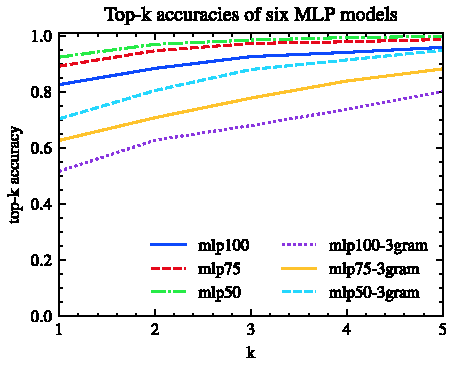
\includegraphics[width=2.5in]{graphics/top_k_mlp_A.pdf}
		\caption{Predictive accruacy}
		\label{fig:top_k_mlp_A}
\end{figure}

\section{Experimental Evaluation}

In this section, we will describe the evaluation of the proposed solutions.  We will verify the effectiveness and limitations of our solutions, and perform a comparative study of different network architectures.  For each network architecture, we will present the benefits and drawbacks, and provide our understanding of the explanation of the observations.

\subsection{Datasets}
The datasets we have used to evaluate our system is a collection of survey data from Statistics Canada, which includes one labour force survey, six COVID-19 surveys, one income survey, one community health survey, and one housing survey.
They offer many real-world characteristics that pose as challenges to  neural network classifiers.  Given the intended application scenarios of our research, we felt that it was important to evaluate our work using real-world datasets. 


These 10 datasets contain both numerical and textual data with different numbers of attributes and tuples. For example, the labour force survey contains data of the Canadian labour market. It has total 60 attributes related to the job market, such as employment status, industry, status of working full-time or part-time, hourly wage, etc. Table \ref{tab:ds01_samples} shows 5 samples with a subset of 10 attributes.

\begin{figure}[t]
	\centering
	\begin{subfigure}{0.45\textwidth}
		\centering
		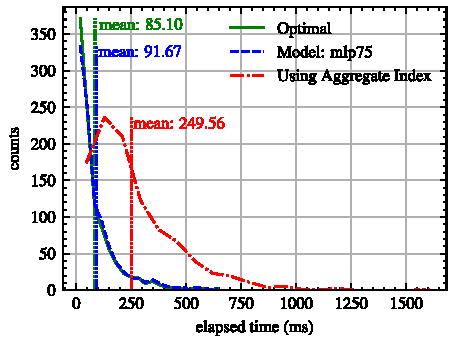
\includegraphics[]{graphics/perf_dist_mlp75_A.pdf}
		\caption{MLP-75-word}
		\label{fig:top_k_mlp_B}
	\end{subfigure}
    \hfill
    \begin{subfigure}{0.45\textwidth}
		\centering
		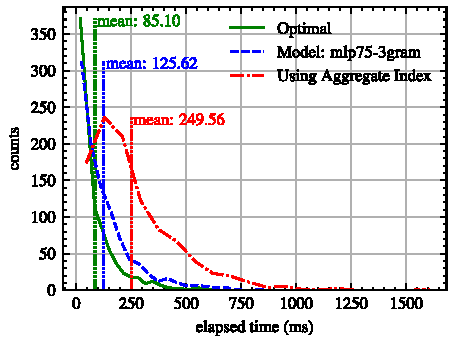
\includegraphics[]{graphics/perf_dist_mlp75_3gram_A.pdf}
		\caption{MLP-75-3gram model}
		\label{fig:perf-mlp75}
	\end{subfigure}
	\caption{Using MLP-75 with word and 3gram tokenization.}
	\label{fig:accuracy-mlp}
\end{figure}

\subsection{Evaluation methodology}
We evaluate five model architectures, including Multilayer Perceptron (MLP), Long Short-Term Memory (LSTM), 1D Convolution (Conv1D), Transformer and MLP-Mixer. We also exam how misspelled keywords affect the models' top-5 accuracies.

We use two metrics for model evaluation. The first metric is query processing time. We submit queries to partitioned indexes and the aggregate index, and record the response times as evaluation benchmark.

The second metric is top-$k$ accuracy. A model's prediction gives us the ordering of Lucene index access. If the Lucene index that a query belongs to is among the top-$k$ of the model's prediction, we consider the prediction accurate.

\begin{table*}[t]
    \centering
    \begin{tabularx}{\textwidth}{|l|X||X|X||X|X|X|}
    \hline
    &    \multicolumn{3}{|c|}{Word tokens} & \multicolumn{3}{|c|}{3-gram tokens} \\ \hline
    Model 
        & parameters
        & $\frac{\mathrm{model}}{\mathrm{optimal}}\ \downarrow$
        & $\frac{\mathrm{model}}{\mathrm{aggr}}\ \downarrow$ 
        & parameters
        & $\frac{\mathrm{model}}{\mathrm{optimal}}\ \downarrow$
        & $\frac{\mathrm{model}}{\mathrm{aggr}}\ \downarrow$
        \\ \hline
    MLP & 3.02M & {\bf 1.10} & 0.37 & 272K & {\bf 1.49} & 0.51\\
    LSTM & 3.05M & 1.52 & 0.52 & 305K & 1.78 & 0.61 \\
    Conv1D & 3.03M & {\bf 1.12} & 0.38 & 277K & 1.68 & 0.57 \\
    Transformer & 3.09M & {\bf 1.12} & 0.38 & 340K & {\bf 1.66} & 0.57 \\
    MLP Mixer & 3.04M & 1.65 & 0.56 & 287K & {\bf 1.65} & 0.56 \\ \hline
    \end{tabularx}
    \caption{Comparison of models under the workload A with the top-3 measurements highlighted.}
    \label{tab:model-comparison}
\end{table*}

\subsection{Query workload generation and tokenization}
\label{subsection:query_workload_gen}
Query workloads are sets of partial tuples. 
We first randomly sample tuples from data reserved for model evaluation. 
Then we apply the same normalization process to them as we do to training datasets. 
After that we convert them to partial tuples by randomly sampling some attributes from them.
We create different workloads by varying the number of attributes sampled.

To create the performance benchmark, we perform search against partitioned indexes and the aggregate index using the constructed partial tuple queries and log the response times. We repeat the process 10 times and compute the mean response times to be used as benchmark for model evaluation. Figure~\ref{fig:perf-mlp75} shows the query evaluation performance between three choices:
\begin{itemize}
\item Optimal case: finding the right index partition immediately.  This is not practically possible as it requires an oracle to perfectly predict which partition to access first.  We include the performance for this case as a theoretical upperbound.
\item Predictive access pattern based on MLP-75 models.
\item Accessing aggregate index without partitioning
\end{itemize}
One can see that the predictive access pattern significantly outperforms
the aggregate index access, and matches the optimal index access when word tokenization is used.

Other architectures (Conv1D, LSTM, Transformers and MLPMixers) have similar performances.  The accelerated query performance lies in the fact that the predictive classifers are quite accurate in predicting which index partition
is more relevant to the query, even by 3-gram tokenization is used.  Figure~\ref{fig:accuracy-mlp} shows the predictive accuracy of the most relevant partition in the top-$k$ results returned by the classifier.

\begin{figure}[h]
	\centering
	\begin{subfigure}{0.45\textwidth}
		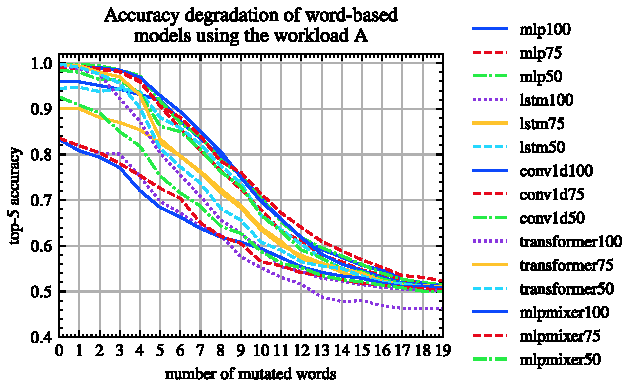
\includegraphics[width=3.5in]{graphics/acc_degradation_word_based_A.pdf}
		\caption{Word-based models}
		\label{fig:acc_degradation_workload_A_word_based}
	\end{subfigure}
	\begin{subfigure}{0.45\textwidth}
		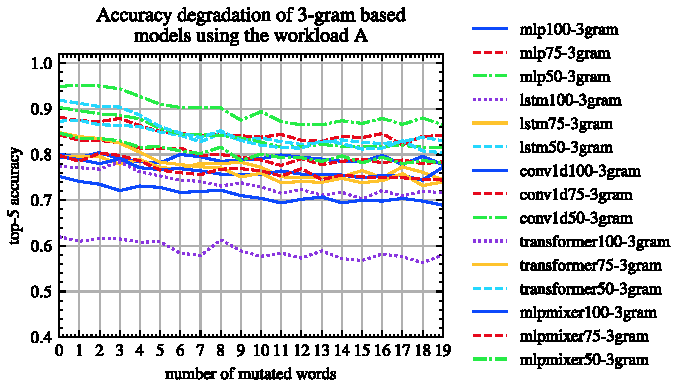
\includegraphics[width=3.5in]{graphics/acc_degradation_3gram_based_A.pdf}
		\caption{3-gram based models}
		\label{fig:acc_degradation_workload_A_3gram}
	\end{subfigure}
	\caption{Top-5 accuracy degradation of all models under the workload A.}
	\label{fig:noisy-queries}
\end{figure}

\subsection{3-gram based models and noisy queries}
In this experiment, we investigate the impact of misspelled words in queries on the models' performance of top-5 accuracy. We simulate the scenario by replacing a randomly selected character in a word with the special character.  The impact of noisy queries on models' performance of top-5 accuracy is shown in Figure\ref{fig:noisy-queries}. The performance degradation of word-based models is much faster than that of 3-gram based models. This clearly shows that 3-gram based models are more resilient to query noises.



\begin{figure}[!th]
	\centering
	\begin{subfigure}[]{0.45\textwidth}
		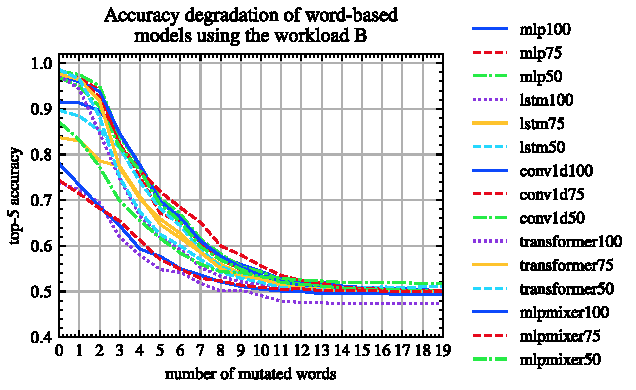
\includegraphics[width=3.5in]{graphics/acc_degradation_word_based_B.pdf}
		\caption{Word-based models}
		\label{fig:acc_degradation_workload_B_word_based}
	\end{subfigure}
	\begin{subfigure}[]{0.45\textwidth}
		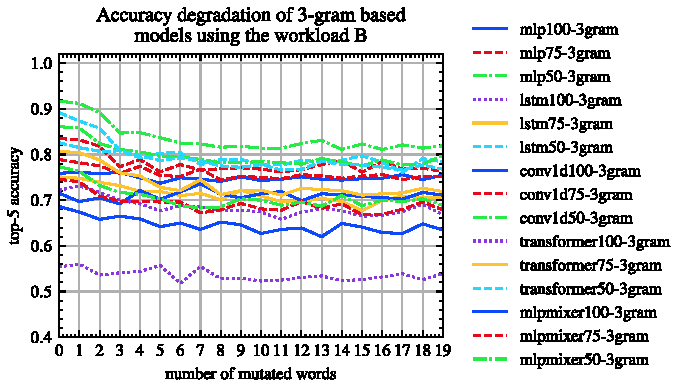
\includegraphics[width=3.5in]{graphics/acc_degradation_3gram_based_B.pdf}
		\caption{3-gram based models}
		\label{fig:acc_degradation_workload_B_3gram}
	\end{subfigure}
	\caption{Top-5 accuracy degradation of all models under the workload B3.}
	\label{fig:acc_degradation_workload_B_all}
\end{figure}

\section{Related Work}

Keyword search is an active area of research starting with DISCOVER \cite{hristidis2002discover}, a system for search relational databases with keyword queries.  Since then, there have been numerous work \cite{yu2022keyword}, extended to fuzzy matching, and to graph databases.

Since the introduction of neural networks and various architectures \cite{DBLP:journals/corr/VaswaniSPUJGKP17,DBLP:journals/corr/abs-2105-01601}, deep learning techniques in text processing \cite{kudo2018sentencepiece,gorishniy2021revisiting,tripathy2021comprehensive} were shown to be highly effective.  Many neural network based solutions had been proposed for tabular data embedding \cite{du2021tabularnet,huang2020tabtransformer,gorishniy2022embeddings,tabbie2021}.  In our work, we demonstrated that such embedding approach can be integrated into keyword query processing pipeline and index optimization.

Neural networks have been applied to learn indexes for multidimensional data \cite{tsunamivldb,DBLP:conf/sigmod/NathanDAK20,ding2020alex}, and for tree structures \cite{ma2022film}.  The use of neural networks for learning indexes has been shown to be effective in reducing the query evaluation time.  In contrast to existing literature, our work focuses on learning the index access pattern for keyword queries.

Fuzzy string matching has been studied in the context of keyword search \cite{DBLP:conf/sigmod/NathanDAK20,DBLP:journals/corr/abs-2105-01601}.  Our work shows that n-gram tokenization provides robust way to form the vocabulary to learn the word embeddings for fuzzy string matching.

\section{Conclusion and Future Work}

We proposed a novel approach to accelerate keyword query processing by learning the index access pattern using neural networks.  We demonstrated that the neural network classifier can be trained to predict the most relevant index partition for a given query.  Our experiments showed that the predictive classifier can significantly reduce the query evaluation time and improve the top-$k$ accuracy.  We also showed that the 3-gram tokenization is more robust to noisy queries than word tokenization.

In the future, we plan to investigate the impact of different tokenization methods on the model's performance.  We also plan to explore the use of reinforcement learning to optimize the index access pattern.  We will also investigate the impact of different query workloads on the model's performance.

% \cite{yu2022keyword,tsunamivldb,ma2022film,DBLP:conf/sigmod/NathanDAK20,DBLP:journals/corr/abs-2012-06678,DBLP:journals/corr/abs-2105-01601,open-data-101,kraska2018case,du2021tabularnet,bordawekar2017using,zhang2019table2vec,huang2020tabtransformer,gorishniy2021revisiting,gorishniy2022embeddings,luo2020network,yin-etal-2020-tabert,tabbie2021,shah2016hash,garcia2005database,marcus2022bao,ding2020alex,kipf2020radixspline,siddiqui2020cost,kudo2018sentencepiece,kim1994fast,lecun2015deep,tripathy2021comprehensive,DBLP:journals/corr/VaswaniSPUJGKP17,tolstikhin2021mlp}

\bibliographystyle{plain}
\bibliography{references.bib}
\end{document}
